% Options for packages loaded elsewhere
\PassOptionsToPackage{unicode}{hyperref}
\PassOptionsToPackage{hyphens}{url}
%
\documentclass[
  ignorenonframetext,
  aspectratio=169,
  ignorenonframetext]{beamer}
\usepackage{pgfpages}
\setbeamertemplate{caption}[numbered]
\setbeamertemplate{caption label separator}{: }
\setbeamercolor{caption name}{fg=normal text.fg}
\beamertemplatenavigationsymbolsempty
% Prevent slide breaks in the middle of a paragraph
\widowpenalties 1 10000
\raggedbottom
\setbeamertemplate{part page}{
  \centering
  \begin{beamercolorbox}[sep=16pt,center]{part title}
    \usebeamerfont{part title}\insertpart\par
  \end{beamercolorbox}
}
\setbeamertemplate{section page}{
  \centering
  \begin{beamercolorbox}[sep=12pt,center]{part title}
    \usebeamerfont{section title}\insertsection\par
  \end{beamercolorbox}
}
\setbeamertemplate{subsection page}{
  \centering
  \begin{beamercolorbox}[sep=8pt,center]{part title}
    \usebeamerfont{subsection title}\insertsubsection\par
  \end{beamercolorbox}
}
\AtBeginPart{
  \frame{\partpage}
}
\AtBeginSection{
  \ifbibliography
  \else
    \frame{\sectionpage}
  \fi
}
\AtBeginSubsection{
  \frame{\subsectionpage}
}
\usepackage{amsmath,amssymb}
\usepackage{lmodern}
\usepackage{iftex}
\ifPDFTeX
  \usepackage[T1]{fontenc}
  \usepackage[utf8]{inputenc}
  \usepackage{textcomp} % provide euro and other symbols
\else % if luatex or xetex
  \usepackage{unicode-math}
  \defaultfontfeatures{Scale=MatchLowercase}
  \defaultfontfeatures[\rmfamily]{Ligatures=TeX,Scale=1}
\fi
% Use upquote if available, for straight quotes in verbatim environments
\IfFileExists{upquote.sty}{\usepackage{upquote}}{}
\IfFileExists{microtype.sty}{% use microtype if available
  \usepackage[]{microtype}
  \UseMicrotypeSet[protrusion]{basicmath} % disable protrusion for tt fonts
}{}
\makeatletter
\@ifundefined{KOMAClassName}{% if non-KOMA class
  \IfFileExists{parskip.sty}{%
    \usepackage{parskip}
  }{% else
    \setlength{\parindent}{0pt}
    \setlength{\parskip}{6pt plus 2pt minus 1pt}}
}{% if KOMA class
  \KOMAoptions{parskip=half}}
\makeatother
\usepackage{xcolor}
\IfFileExists{xurl.sty}{\usepackage{xurl}}{} % add URL line breaks if available
\IfFileExists{bookmark.sty}{\usepackage{bookmark}}{\usepackage{hyperref}}
\hypersetup{
  pdftitle={Determinantes do spread ex-post e rentabilidade bancária: Um modelo em painel dinâmico com vetores autorregressivos e estimação por método de momentos generalizados},
  pdfauthor={JACKSON DA SILVA TORRES},
  hidelinks,
  pdfcreator={LaTeX via pandoc}}
\urlstyle{same} % disable monospaced font for URLs
\newif\ifbibliography
\usepackage{longtable,booktabs,array}
\usepackage{calc} % for calculating minipage widths
\usepackage{caption}
% Make caption package work with longtable
\makeatletter
\def\fnum@table{\tablename~\thetable}
\makeatother
\setlength{\emergencystretch}{3em} % prevent overfull lines
\providecommand{\tightlist}{%
  \setlength{\itemsep}{0pt}\setlength{\parskip}{0pt}}
\setcounter{secnumdepth}{-\maxdimen} % remove section numbering
\usepackage[utf8]{inputenc} % codificacao de caracteres
\usepackage[T1]{fontenc}    % codificacao de fontes
\usepackage[brazil]{babel}  % idioma
\usepackage{graphicx}       %fundo
\usetheme{default}          % tema
\usecolortheme{orchid}     % cores
\usefonttheme[onlymath]{serif} % fonte modo matematico
\usepackage{wallpaper}

\usepackage{tikz}

\usepackage[
style=abnt,
backref=true,
backend=biber,
maxcitenames=2,
%citecounter=true,
backrefstyle=three,
%nohashothers=true
]{biblatex}

%\setbeameroption{show notes}
%\setbeameroption{show notes on second screen=right}

%\usepackage[pdftex]{graphicx}

\usepackage[final]{pdfpages}

\usepackage{booktabs}

\usepackage{helvet}
\renewcommand{\familydefault}{\sfdefault}
\makeindex
\DeclareUnicodeCharacter{0301}{******}
\DeclareUnicodeCharacter{0303}{******}
\DeclareUnicodeCharacter{0327}{******}
\DeclareUnicodeCharacter{0302}{******}
\ifLuaTeX
  \usepackage{selnolig}  % disable illegal ligatures
\fi
\newlength{\cslhangindent}
\setlength{\cslhangindent}{1.5em}
\newlength{\csllabelwidth}
\setlength{\csllabelwidth}{3em}
\newenvironment{CSLReferences}[2] % #1 hanging-ident, #2 entry spacing
 {% don't indent paragraphs
  \setlength{\parindent}{0pt}
  % turn on hanging indent if param 1 is 1
  \ifodd #1 \everypar{\setlength{\hangindent}{\cslhangindent}}\ignorespaces\fi
  % set entry spacing
  \ifnum #2 > 0
  \setlength{\parskip}{#2\baselineskip}
  \fi
 }%
 {}
\usepackage{calc}
\newcommand{\CSLBlock}[1]{#1\hfill\break}
\newcommand{\CSLLeftMargin}[1]{\parbox[t]{\csllabelwidth}{#1}}
\newcommand{\CSLRightInline}[1]{\parbox[t]{\linewidth - \csllabelwidth}{#1}\break}
\newcommand{\CSLIndent}[1]{\hspace{\cslhangindent}#1}

\title{Determinantes do \textbf{spread ex-post} e rentabilidade
bancária: Um modelo em painel dinâmico com vetores autorregressivos e
estimação por método de momentos generalizados}
\author{JACKSON DA SILVA TORRES}
\date{30 DE JUNHO DE 2021}

\begin{document}
\frame{\titlepage}

\begin{frame}{\textbf{SUMÁRIO }}
\protect\hypertarget{sumuxe1rio}{}
\begin{columns}[T]
\begin{column}{0.6\textwidth}
\begin{enumerate}
\item
  \textbf{INTRODUÇÃO}

  \begin{enumerate}
  \item
    CONTEXTUALIZAÇÃO
  \item
    OBJETIVOS
  \item
    JUSTIFICATIVA TEÓRICA E PRÁTICA
  \item
    ESTRUTURA DA DISSERTAÇÃO
  \end{enumerate}
\item
  \textbf{REFERENCIAL TEÓRICO}

  \begin{enumerate}
  \item
    SETOR BANCÁRIO NO BRASIL
  \item
    SPREAD BANCÁRIO
  \item
    ESTUDOS ANTERIORES
  \end{enumerate}
\end{enumerate}
\end{column}

\begin{column}{0.4\textwidth}
\begin{enumerate}
\setcounter{enumi}{2}
\item
  \textbf{PROCEDIMENTOS METODOLÓGICOS}
\item
  \textbf{RESULTADOS}
\item
  \textbf{CONSIDERAÇÕS FINAIS}
\end{enumerate}
\end{column}
\end{columns}
\end{frame}

\begin{frame}{\textbf{1.1 CONTEXTUALIZAÇÃO}}
\protect\hypertarget{contextualizauxe7uxe3o}{}
\begin{enumerate}
[a.]
\item
  \textbf{\emph{Spread}} como indicador de \textbf{desempenho da
  economia} (\protect\hyperlink{ref-WB:2005}{BANK and IMF 2005};
  \protect\hyperlink{ref-levine:1997}{Levine 1997};
  \protect\hyperlink{ref-dantas:2012}{Dantas 2012};
  \protect\hyperlink{ref-leal:2006}{Souza 2006})

  \begin{itemize}
  \item
    \textbf{Elevados níveis} de \textbf{\emph{Spread}} atuam no
    \textbf{desfavorecimento do crédito}.
  \item
    Fundo Monetário Internacional (FMI) e Banco Mundial (BM) realizam e
    incentivam estudos sobre o indicador a nível mundial
    {[}\protect\hyperlink{ref-WB:2005}{BANK and IMF}
    (\protect\hyperlink{ref-WB:2005}{2005}).

    \begin{itemize}
    \tightlist
    \item
      A maioria indica a \textbf{relação inversa} entre
      \textbf{\emph{Spread}} e \textbf{desenvolvimento econômico}
    \end{itemize}
  \end{itemize}
\item
  \textbf{\emph{Spread}} como \textbf{indicador de eficência} do
  \textbf{Sistema Financeiro}\\
  (\protect\hyperlink{ref-levine:1997}{Levine 1997};
  \protect\hyperlink{ref-dantas:2012}{Dantas 2012};
  \protect\hyperlink{ref-leal:2006}{Souza 2006})

  \begin{itemize}
  \tightlist
  \item
    Relacionado com a \textbf{solidez} e \textbf{competitividade} das
    instituições
  \end{itemize}
\end{enumerate}

\textcolor{blue}{DESENVOLVIMENTO ECONÔMICO X SISTEMA FINANCEIRO SÓLIDO}
\end{frame}

\begin{frame}{\textbf{1.2 OBJETIVOS}}
\protect\hypertarget{objetivos}{}
\textbf{OBJETIVO GERAL}

\begin{enumerate}
\tightlist
\item
  Investigar variáveis microeconômicas e macroeconômicas que exerçam
  influência significativa sobre o \emph{spread ex-post} e como estas
  afetaram a rentabilidade das instituições bancárias brasileiras, entre
  março de 2011 e novembro de 2020.
\end{enumerate}
\end{frame}

\begin{frame}{\textbf{1.2 OBJETIVOS}}
\protect\hypertarget{objetivos-1}{}
\textbf{OBJETIVOS ESPECÍFICOS}

\begin{enumerate}
\item
  \textbf{Realizar} o mapeamento e sistematização de aspectos teóricos e
  técnicos sobre o setor bancário e \emph{spread} no Brasil;
\item
  \textbf{Identificar} e testar variáveis macroeconômicas e
  microeconômicas enquanto componentes implícitos e explícitos de
  determinação do \textbf{\emph{Spread}} bancário \textbf{ex-post};
\item
  Analisar como as variações das variáveis determinantes do
  \textbf{\emph{Spread}} bancário afetaram a rentabilidade dos bancos.
\end{enumerate}
\end{frame}

\begin{frame}{\textbf{1.3 JUSTIFICATIVA TEÓRICA E PRÁTICA}}
\protect\hypertarget{justificativa-teuxf3rica-e-pruxe1tica}{}
\begin{itemize}
\item
  \textbf{Evidências} da \textbf{influência} do nível de
  \textbf{\emph{Spread}} no desenvolvimento econômico.
\item
  \textbf{Importância} do \textbf{\emph{Spread}} na \textbf{solidez} do
  \textbf{sistema financeiro}.
\item
  \textbf{Economia} e \textbf{Mercado Financeiro} em \textbf{constantes
  transformações}.
\item
  O \textbf{cenário brasileiro} é \textbf{considerado peculiar} por
  possuir histórico de (\protect\hyperlink{ref-levine:1997}{Levine
  1997}; \protect\hyperlink{ref-matos:2003}{Matos 2003}):

  \begin{itemize}
  \item
    \textbf{Elevados níveis} de \textbf{\emph{Spread}} bancário
  \item
    \textbf{Baixa relação} entre \textbf{crédito e PIB}
  \item
    \textbf{Cenários} de \textbf{crescimento econômico}
    \textbf{instáveis} e considerados \textbf{baixos}
  \end{itemize}
\item
  \textbf{Carências} de \textbf{pesquisas} acerca do
  \textbf{\emph{Spread ex-post}}
\item
  Existência de lacunas, divergências e incogluências de pesquisas.
\end{itemize}
\end{frame}

\begin{frame}{\textbf{2.1 SETOR BANCÁRIO NO BRASIL}}
\protect\hypertarget{setor-bancuxe1rio-no-brasil}{}
\begin{columns}[T]
\begin{column}{0.5\textwidth}
\begin{itemize}
\item
  \textbf{Contexto Histórico}
\item
  \textbf{Evolução}
\item
  \textbf{Organização}

  \begin{itemize}
  \tightlist
  \item
    Sistema Financeiro Nacional
  \item
    Órgãos Normativos
  \item
    Órgão Supervisores
  \item
    Operadores

    \begin{itemize}
    \tightlist
    \item
      Bancos e Caixas Econômicas
    \item
      Banco Comercial
    \item
      Banco de Investimento
    \item
      Banco de Desenvolvimento
    \item
      Banco de Câmbio
    \item
      Banco Múltiplos
    \item
      Caixa Econômica
    \end{itemize}
  \end{itemize}
\end{itemize}
\end{column}

\begin{column}{0.5\textwidth}
\begin{itemize}
\tightlist
\item
  \textbf{Características}

  \begin{itemize}
  \tightlist
  \item
    Concentração Bancária
  \item
    Tendência para domínio da participação estrangeira
  \item
    Elevados níveis de \emph{Spread} bancário
  \item
    Histórico de baixa relação Crédito/PIB
  \item
    Histórico de crescimento instável
  \end{itemize}
\end{itemize}
\end{column}
\end{columns}
\end{frame}

\begin{frame}{\textbf{2.1 SETOR BANCÁRIO NO BRASIL}}
\protect\hypertarget{setor-bancuxe1rio-no-brasil-1}{}
\begin{center}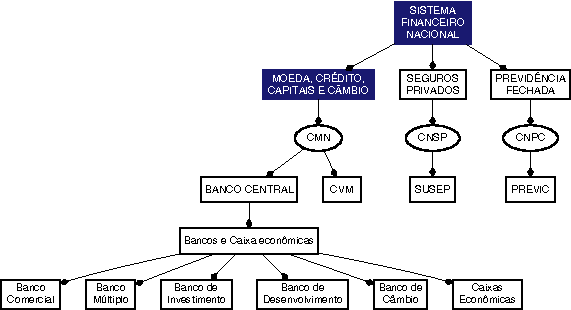
\includegraphics{02-final_presentation-V1_files/figure-beamer/diagram.sfn-1} \end{center}
\end{frame}

\begin{frame}{\textbf{2.2 SPREAD BANCÁRIO}}
\protect\hypertarget{spread-bancuxe1rio}{}
\begin{itemize}
\tightlist
\item
  \textbf{CONCEITOS}

  \begin{itemize}
  \tightlist
  \item
    O termo \emph{spread} significa --- tradução livre ---
    \textbf{amplitude}, \textbf{crescimento} e \textbf{extensão}.
  \item
    Utilizado no \textbf{setor financeiro} no sentido de \textbf{margem}
  \item
    É obtido através da \textbf{diferença} entre a \textbf{taxa de
    aplicação} e a \textbf{taxa de captação}

    \begin{itemize}
    \tightlist
    \item
      Diferença entre custos operacionais
      (\protect\hyperlink{ref-BCB:2016}{BACEN 2016})
      (\protect\hyperlink{ref-BCB:2000}{BACEN 2000}).
    \end{itemize}
  \end{itemize}
\end{itemize}

\[ 
\textbf{Spread} = \textbf{Taxa de Aplicação} - \textbf{Taxa de Captação}
\] \[
\textbf{Spread} = \textbf{Juros Tomador} - \textbf{Juros Investidor}
\]

\begin{itemize}
\tightlist
\item
  O \textbf{\emph{Spread}} bancário representa uma medida que sinaliza o
  desempenho dos bancos (\protect\hyperlink{ref-levine:1997}{Levine
  1997}) e indicador de eficiência da
  economia(\protect\hyperlink{ref-WB:2005}{BANK and IMF 2005}).
\end{itemize}
\end{frame}

\begin{frame}{\textbf{2.2 SPREAD BANCÁRIO}}
\protect\hypertarget{spread-bancuxe1rio-1}{}
\begin{columns}[T]
\begin{column}{0.5\textwidth}
\textbf{ÓTICAS} (\protect\hyperlink{ref-dick:1999}{Dick 1999})

\begin{center}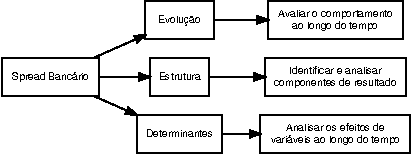
\includegraphics{02-final_presentation-V1_files/figure-beamer/diagram.otic-1} \end{center}
\end{column}

\begin{column}{0.5\textwidth}
\textbf{CARACTERÍSTICAS} (\protect\hyperlink{ref-leal:2006}{Souza 2006})

\begin{center}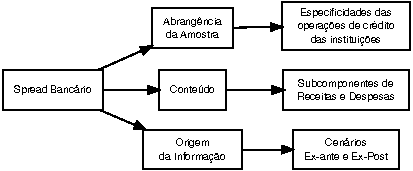
\includegraphics{02-final_presentation-V1_files/figure-beamer/diagram.carac-1} \end{center}
\end{column}
\end{columns}

\textbf{DIMENSÃO}

\begin{center}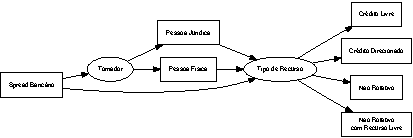
\includegraphics{02-final_presentation-V1_files/figure-beamer/d.spread.dim-1} \end{center}
\end{frame}

\begin{frame}{\textbf{2.2 SPREAD BANCÁRIO}}
\protect\hypertarget{spread-bancuxe1rio-2}{}
\textbf{VOLUME-PRAZO-RISCO}

\begin{center}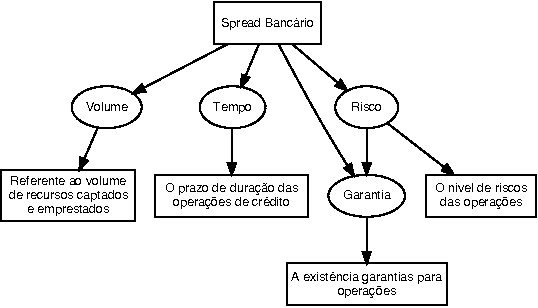
\includegraphics{02-final_presentation-V1_files/figure-beamer/diagram.spread.vol.tem.ris-1} \end{center}
\end{frame}

\begin{frame}{\textbf{2.2.2 SPREAD BANCÁRIO NO BRASIL}}
\protect\hypertarget{spread-bancuxe1rio-no-brasil}{}
\begin{itemize}
\item
  Séries mantidas pelo Banco Central:

  \begin{itemize}
  \item
    \textbf{Spread} Médio das operações de crédito (MOC)
  \item
    \textbf{Spread} do Indicador de Custo de Crédito (ICC)
  \end{itemize}
\item
  Componentes explícitos do \textbf{Spread}
  (\protect\hyperlink{ref-BCB:2000}{BACEN 2000}):

  \begin{itemize}
  \item
    Inadimplência (\(Ind\))
  \item
    Despesas administrativas (\(DA\))
  \item
    Impostos diretos (\(ID\)) e indiretos (\(II\))
  \item
    Custo de captação (\(CP\))
  \item
    Margem de lucro (\(ML\))
  \end{itemize}
\end{itemize}
\end{frame}

\begin{frame}{\textbf{2.2.2 SPREAD BANCÁRIO NO BRASIL}}
\protect\hypertarget{spread-bancuxe1rio-no-brasil-1}{}
\begin{itemize}
\tightlist
\item
  Considerável diferença entre os spread por tipo de tomador e tipo de
  crédito
\end{itemize}

\begin{center}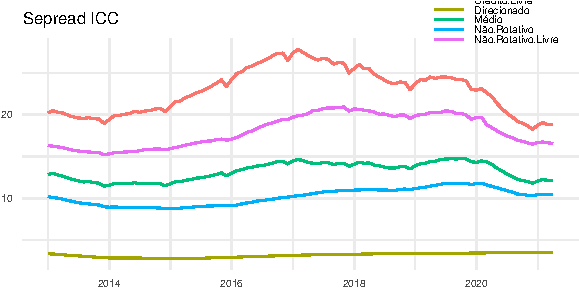
\includegraphics{02-final_presentation-V1_files/figure-beamer/spread.icc-1} \end{center}
\end{frame}

\begin{frame}{\textbf{2.2.2 SPREAD BANCÁRIO NO BRASIL}}
\protect\hypertarget{spread-bancuxe1rio-no-brasil-2}{}
\textbf{ESTUDOS EMPÍRICOS}

\begin{itemize}
\item
  Na \textbf{literatura acadêmica} \textbf{não existe} uma
  \textbf{teoria formalizada} acerca do \textbf{\emph{Spread}} bancário
  (\protect\hyperlink{ref-timotio:2018}{Magalhães-Timotio 2018})
\item
  A \textbf{grande maioria} dos \textbf{estudos} realizados no Brasil
  \textbf{utilizam} as medidas de \textbf{\emph{Spread}} bancário
  divulgadas pelo Banco Central, que remetem a uma perspectiva
  \textbf{\emph{ex-ante}} (\protect\hyperlink{ref-dantas:2012}{Dantas
  2012})
\item
  Estudos empíricos \textbf{\emph{spread ex-post}}:

  \begin{itemize}
  \tightlist
  \item
    GUIMARÃES (2002)
  \item
    DANTAS (2012)
  \item
    ALMEIDA (2013)
  \item
    TIMOTIO (2018)
  \end{itemize}
\end{itemize}
\end{frame}

\begin{frame}{\textbf{2.2.2 SPREAD BANCÁRIO NO BRASIL}}
\protect\hypertarget{spread-bancuxe1rio-no-brasil-3}{}
\textbf{VARIÁVEIS IDENTIFICADAS}

\begin{columns}[T]
\begin{column}{0.5\textwidth}
\begin{itemize}
\tightlist
\item
  Modalidade de Instituições
\item
  Controle de Capital
\item
  Relação Crédito/PIB
\item
  Saldo da carteira de crédito
\item
  Indicador do Custo de Crédito
\item
  Selic
\item
  Depósitos Compulsórios
\item
  Despesas Operacionais
\end{itemize}
\end{column}

\begin{column}{0.5\textwidth}
\begin{itemize}
\tightlist
\item
  Inadimplência
\item
  Risco de Crédito
\item
  Dados contábeis padronizadados
\item
  Base Monetária
\item
  Agregados Monetários
\item
  Velocidade da Moeda
\item
  Selic
\item
  Índice HHI - Concentração
\end{itemize}
\end{column}
\end{columns}
\end{frame}

\begin{frame}{\textbf{3. PROCEDIMENTOS METODOLÓGICOS}}
\protect\hypertarget{procedimentos-metodoluxf3gicos}{}
\textbf{FERRAMENTAS}

\begin{itemize}
\item
  Trabalho foi desenvolvido e editado em ambiente \textbf{R Markdown}
\item
  Utilização de linguagem \textbf{Latex} para padronização de textos,
  figuras e tabelas
\item
  Linguagens \textbf{R} e \textbf{Python} para coleta, tratamento
  modelagem e estimação dos conjuntos de dados.
\item
  Utilizados e construídos \textbf{frameworks}
\end{itemize}
\end{frame}

\begin{frame}{\textbf{3. PROCEDIMENTOS METODOLÓGICOS}}
\protect\hypertarget{procedimentos-metodoluxf3gicos-1}{}
\textbf{DELIMITAÇÃO DOS DADOS}

\begin{itemize}
\item
  Serão selecionadas a ``população'' de instituições bancárias das
  modalidades:

  \begin{itemize}
  \tightlist
  \item
    Banco Múltiplo
  \item
    Banco Comercial
  \item
    Banco de Investimento
  \item
    Banco de Desenvolvimento
  \item
    Caixas Econômicas
  \end{itemize}
\item
  Período entre março 2011 e o novembro de 2020.
\item
  Dados serão obtidos de forma secundária nos bancos de dados abertos do
  Banco Central, IPEA e IBGE e CVM
\end{itemize}
\end{frame}

\begin{frame}{\textbf{3. PROCEDIMENTOS METODOLÓGICOS}}
\protect\hypertarget{procedimentos-metodoluxf3gicos-2}{}
\textbf{RESUMO DE DADOS}

\begin{longtable}[]{@{}llll@{}}
\toprule
\textbf{Nome} & \textbf{Código} & \textbf{Periodicidade} &
\textbf{Fonte} \\
\midrule
\endhead
Dados Financeiros & 370 & Mensal & Banco Central \\
PIB & BM12\_PIB12 & Mensal & IPEA \\
Selic Over & BM12\_TJOVER12 & Mensal & Banco Central \\
Meios de Pagamentos & BM12\_M4NCN12 & Mensal & IPEA \\
IPCA & PRECOS12\_IPCAG12 & Mensal & IPEA \\
Compulsório Poupança & 1848 & Mensal & Banco Central \\
Compulsório a vista & 1849 & Mensal & Banco Central \\
Compulsório a prazo & 1850 & Mensal & Banco Central \\
Base Monetária Ampliada & 1833 & Mensal & Banco Central \\
\bottomrule
\end{longtable}
\end{frame}

\begin{frame}{\textbf{3. PROCEDIMENTOS METODOLÓGICOS}}
\protect\hypertarget{procedimentos-metodoluxf3gicos-3}{}
Para fins de modelagem, o \emph{spread} será abordado dentro do conceito
de precificação, seguindo a decomposição desenvolvida no APÊNDICE A a
partir da forma tautógica (\autoref{eq:taut}), na forma da equação
\autoref{eq:amor100} e dos componentes da taxa de juros conforme a
equação \autoref{eq:txjur100}.

\begin{equation}\label{eq:taut}
Spr = i_{apl} - i_{cap} 
\end{equation}

\begin{columns}[T]
\begin{column}{0.6\textwidth}
\begin{itemize}
\tightlist
\item
  Período de tempo (\(n\))
\item
  Tipo de tomador (\(a\))
\item
  Tipo de recurso (\(b\))
\item
  Modalidade de operação (\(c\))
\end{itemize}
\end{column}

\begin{column}{0.4\textwidth}
\begin{itemize}
\tightlist
\item
  Parcela de receita futura (\(ROP_{n}\))
\item
  Tipo de operação (\(d\)) e origem do capital(\(e\)).
\item
  Sensibilidades de Volume (\(v\)), Prazo (\(p\)), Risco (\(r\)) e
  Garantia (\(g\))
\end{itemize}
\end{column}
\end{columns}
\end{frame}

\begin{frame}{\textbf{3. PROCEDIMENTOS METODOLÓGICOS}}
\protect\hypertarget{procedimentos-metodoluxf3gicos-4}{}
\begin{equation}\label{eq:amor100}
SprEp_{[n,a,b,c,d,e]} = \left[ \frac{ROp_{n}[\frac{   ijr_{}  }{  [1 + ijr_{}]^n -1  }]}{Op_{n}} -1 \right] - \left[ \frac{DC_{n}}{C_{n}} \right]
\end{equation}

\begin{equation}\label{eq:txjur100}
\begin{aligned}
ijr_{[t(a,b,c,d,e)]} = & \frac{[i_{adm} + i_{Inad} + i_{IOF} + r +  \frac{(i_{cap} + i_{fgc} + i_{ac}.i_{comp} - i_{r}.i_{fgc}+ i_{cs}.i_{fgc})}{1 - i_{comp} - i_{fgc}}]}
{[1 - (\frac{i_{ll}}{1 - i_{r} - i_{cs}} + i_{pis}.(1 - i_{r} - i_{cs}) + i_{cof}.(1 - i_{r} - i_{cs}) + 0,99i_{r} + i_{cs})]}v'p'g'
\end{aligned}
\end{equation}
\end{frame}

\begin{frame}{\textbf{3. PROCEDIMENTOS METODOLÓGICOS}}
\protect\hypertarget{procedimentos-metodoluxf3gicos-5}{}
\begin{itemize}
\tightlist
\item
  Foram testados métodos SUR: \emph{Pooling}, Efeitos Fixos e Efeitos
  Aleatórios

  \begin{itemize}
  \tightlist
  \item
    Os resultados apresentaram heterocedasticidade e correlação
  \end{itemize}
\item
  Testes de dependência \emph{cross-seccional} e correlação serial não
  significam essencialmente que exista essa condição para o modelo
  (\protect\hyperlink{ref-sargan:1964}{Sargan 1964}) e
  (\protect\hyperlink{ref-hendry:1978}{Hendry and Mizon 1978})

  \begin{itemize}
  \tightlist
  \item
    Mas um problema de especificação dinâmica, com a omissão de
    variáveis defasadas.
  \end{itemize}
\end{itemize}
\end{frame}

\begin{frame}{\textbf{3. PROCEDIMENTOS METODOLÓGICOS}}
\protect\hypertarget{procedimentos-metodoluxf3gicos-6}{}
\begin{itemize}
\tightlist
\item
  Foi identificada a metodologia de painel de vetores autoregressivos
  (PVAR) (\protect\hyperlink{ref-sigmund:2008}{Sigmund and Ferstl 2008})

  \begin{itemize}
  \tightlist
  \item
    Comporta mais de uma variável dependente defasada
  \item
    Variáveis preditoras endógenas
  \item
    Variáveis preditoras exógenas
  \item
    Estimação por método de momentos generalizados (GMM),
  \item
    Transformação \emph{Forward orthogonal deviations}
  \item
    Duas etapas
  \end{itemize}
\end{itemize}

\begin{equation}\label{eq:pvar}
\mathbf{W}_{it} = \mathbf{a}_{i} + \Phi \mathbf{W}_{i, t-1} + \epsilon_{it}  
\end{equation}
\end{frame}

\begin{frame}{\textbf{3. PROCEDIMENTOS METODOLÓGICOS}}
\protect\hypertarget{procedimentos-metodoluxf3gicos-7}{}
\begin{itemize}
\tightlist
\item
  O modelo PVAR-GMM (System) de
  (\protect\hyperlink{ref-blundelbond:1998}{Blundell and Bond 1998})
  (\autoref{eq:pvarsys})

  \begin{itemize}
  \tightlist
  \item
    Atua corrigindo o viés causado pelos efeitos fixos aplicados em
    painéis dinâmicos

    \begin{itemize}
    \tightlist
    \item
      Através da modificação, ou seja, a retirada em primeira ordem, dos
      instrumentos, passando a serem exógenos aos efeitos fixos
    \item
      Assumindo que as variações nas variáveis instrumentais não são
      correlacionadas com os efeitos fixos e com o erro.
    \end{itemize}
  \end{itemize}
\end{itemize}

\begin{equation}
\mathbf{W}_{it} - \Phi\mathbf{W}_{i, t-1} = \mathbf{a}_{i} + \epsilon_{it}  
\end{equation}
\end{frame}

\begin{frame}{\textbf{3. PROCEDIMENTOS METODOLÓGICOS}}
\protect\hypertarget{procedimentos-metodoluxf3gicos-8}{}
\begin{itemize}
\item
  De acordo com (\protect\hyperlink{ref-bontempi:2015}{Bontempi and
  Mammi 2000}) os modelos PVAR-GMM apresentam problema proliferação de
  instrumentos.

  \begin{itemize}
  \tightlist
  \item
    Geram sobreajuste das preditoras endógenas
  \item
    Viés nas variáveis instrumentais estimadores GMM
  \item
    Enfraquecimento do poder dos testes de superidentificação.
  \end{itemize}
\item
  Para tal problema (\protect\hyperlink{ref-bontempi:2015}{Bontempi and
  Mammi 2000}) defendem utilização da análise de componentes principais
  (PCA).
\item
  Os instrumentos PCA atuam
  (\protect\hyperlink{ref-bontempi:2015}{Bontempi and Mammi 2000}):

  \begin{itemize}
  \tightlist
  \item
    reduzindo os instrumentos disponíveis,
  \item
    reescrevendo as informações transmitidas por variáveis altamente
    correlacionadas em termos de um conjunto de combinações lineares
    ortogonais ideais das variáveis originais

    \begin{itemize}
    \tightlist
    \item
      retendo um número menor deles, sumarizando o painel e formando um
      espécie de índice-resumo .
    \end{itemize}
  \end{itemize}
\end{itemize}
\end{frame}

\begin{frame}{\textbf{3. PROCEDIMENTOS METODOLÓGICOS}}
\protect\hypertarget{procedimentos-metodoluxf3gicos-9}{}
\begin{itemize}
\tightlist
\item
  O modelo PVAR-GMM (System) será testado pelo método J-Hansen,

  \begin{itemize}
  \tightlist
  \item
    Analisa a superidentificação de restrições (\emph{overidentifying
    restrictions}), gerando a estatística J.
  \item
    A hipotese nula é a validade de todas a variáveis do modelo, através
    do teste Qui Quadrado e seu respectivo valor P.
  \end{itemize}
\end{itemize}

\begin{equation}\label{eq:jhansen}
J_{n}(b,c) = n \hspace{10pt} \text{inf}_{\theta_{[b]} \in \theta_{[b]}} G_{nc} (\Theta_{[b]})^{'}W_{nc}(b,c)G_{nc}(\Theta_{[b]}) 
\end{equation}
\end{frame}

\begin{frame}{\textbf{3. PROCEDIMENTOS METODOLÓGICOS}}
\protect\hypertarget{procedimentos-metodoluxf3gicos-10}{}
\begin{itemize}
\tightlist
\item
  Será utilizado modelo consistente de critérios de seleção de momento
  (MMSC)

  \begin{itemize}
  \tightlist
  \item
    Desenvolvido por (\protect\hyperlink{ref-andrews-lu:2001}{Andrews
    and Lu 2000}), baseado no teste J-Hansen para superidentificação de
    restrições,
  \item
    Nos Critério Bayesiano de Schwarz (BIC)
  \item
    Critério de informação Hannan--Quinn (HQIC)
  \item
    Critério de informação de Akaike (AIC),\\
  \end{itemize}
\item
  Indicado para modelos em painéis dinâmicos, para efeitos fixos não
  observados, estimados por GMM
  (\protect\hyperlink{ref-sigmund:2008}{Sigmund and Ferstl 2008})
  (\protect\hyperlink{ref-zivotwang:2003}{Zivot and Wang 2003}).
\end{itemize}

\begin{equation}\label{eq:andrewslu}
\begin{aligned}{}
& MMSC-BIC = k_{n} = \ln n \hspace{10pt} \text{and} \hspace{10pt} MMSC_{BIC,n}(b,c) = J_{n}(b,c) — (|c| - |b| )ln,n \\
& MMSC-AIC = k_{n} = 2 \hspace{10pt} \text{and} \hspace{10pt} 
MMSC_{AIC,n}(b,c) = J_{n}(b,c) — 2(|c| - |b| ) \\
& MMSC-HQIC = k_{n} = Q \ln \ln n  \hspace{10pt} \text{for some} \hspace{10pt} Q > 2 \hspace{10pt} \hspace{10pt} \text{and} \hspace{10pt}  \\
& MMSC_{HQIC,n}(b,c) = J_{n}(b,c) — Q(|c| - |b|)\ln\ln n
\end{aligned}
\end{equation}
\end{frame}

\begin{frame}{\textbf{3. PROCEDIMENTOS METODOLÓGICOS}}
\protect\hypertarget{procedimentos-metodoluxf3gicos-11}{}
\begin{itemize}
\tightlist
\item
  O modelo PVAR-GMM System será avaliado pela condição de estabilidade
  padrão dos coeficientes VAR do painel,

  \begin{itemize}
  \tightlist
  \item
    Baseado no módulo de cada valor próprio do modelo estimado.
  \item
    Um modelo VAR é estável se todos os módulos da matriz par forem
    estritamente menores que um.
  \item
    A estabilidade implica que o painel VAR é invertível e tem uma
    representação de média móvel vetorial de ordem infinita.
  \end{itemize}
\end{itemize}
\end{frame}

\begin{frame}{\textbf{3. PROCEDIMENTOS METODOLÓGICOS}}
\protect\hypertarget{procedimentos-metodoluxf3gicos-12}{}
Para a análise do modelo PVAR-GMM (System) será utilizada a função
impulso resposta octogonal (OIRF) - Visando analisar a resposta de uma
variável ao impulsos das demais variável de forma isolada dentro da
mesma equação - Eliminando desta forma o problema de correlação
endógena, que ocorre no método de impulso resposta convencional (IRF)
(\protect\hyperlink{ref-sigmund:2008}{Sigmund and Ferstl 2008})

\begin{equation}\label{eq:oirf}
OIRF(k,r) = \frac{\delta\mathbf{W}_{i,t+k}}{\delta(\mathbf{u}_{it})_{r}} = \mathbf{\Theta}_{k}\mathbf{e}_{r}  
\end{equation}
\end{frame}

\begin{frame}{\textbf{3. PROCEDIMENTOS METODOLÓGICOS}}
\protect\hypertarget{procedimentos-metodoluxf3gicos-13}{}
\begin{itemize}
\tightlist
\item
  Os intervalos de confiança para as análises das funções impulso
  reposta OIRF serão construídos através do procedimento de
  \emph{bootstrap cross-sectional}
\end{itemize}
\end{frame}

\begin{frame}{\textbf{3. PROCEDIMENTOS METODOLÓGICOS}}
\protect\hypertarget{procedimentos-metodoluxf3gicos-14}{}
\textbf{MODELO}

O modelo PVAR-GMM a ser construído se baseia na hipótese que o
\emph{spread ex-post} (\(y'\)) e rentabilidade (\(y''\)), utilizadas
como preditoras com (\(p\)) defasagens, são determinados diante um
conjunto de variáveis endógenas (\(m\)) representando suas
cateterísticas operacionais e um conjunto de variáveis exógenas (\(n\)),
diante do tempo (\(\eta\)), conforme representado na equação
\autoref{eq:modelfinal}

\begin{equation}\label{eq:modelfinal}
\begin{aligned}
y_{it} = & \alpha y_{it-1}+ \cdots +\alpha y_{it-p} + \beta_{DAdm} +  \beta_{DesCap} + \beta_{OtDes} + \beta_{Inad} + \beta_{RcPd} + \beta_{EPr} \\ 
& + \beta_{DepAv} + \beta_{DepAp} + \beta_{DepPop} + \beta_{ROpCr} + \beta_{RSrv} + \beta_{RPart} + \beta_{OtROp} + \beta_{OpEmp} \\
& + \beta_{OpFin} + \beta_{tOp} + \beta_{ImpInd} + \beta_{Rend} + \gamma_{SelOvr} + \gamma_{VelMo} + \gamma_{Comp} + \gamma_{GrCon} + \gamma_{IPCA}  \\ 
& + \gamma_{lnBMA} + \gamma_{lnOpCrMkt} + \eta_{i} + \phi_{t} + \epsilon_{it} 
\end{aligned}
\end{equation}
\end{frame}

\begin{frame}{\textbf{3. PROCEDIMENTOS METODOLÓGICOS}}
\protect\hypertarget{procedimentos-metodoluxf3gicos-15}{}
\(SprEp_{it}\): O \emph{Spread Ex-post} (\(SprEp\)) será calculado a
partir dos resultados contábeis, resultante da diferença entre a relação
de receitas operacionais (\(RcOp\) --- Conta 71000008) e operações de
crédito média (\(OpCrMe\) --- Conta 16000001), e a relação de despesas
de captação (\(DesCap\) --- Conta 81100008 ) e depósitos médio (\(Dep\)
--- Conta 41000007).

\begin{equation}\label{eq:sprbase}
SprEp_{it} = \frac{RcOp_{it}}{\frac{1}{2}(OpCr_{it} + OpCr_{it-1}) } - \frac{DesCap_{it}}{\frac{1}{2}(Dep_{it} + Dep_{it-1})}
\end{equation}
\end{frame}

\begin{frame}{\textbf{3. PROCEDIMENTOS METODOLÓGICOS}}
\protect\hypertarget{procedimentos-metodoluxf3gicos-16}{}
\(Rent\): A rentabilidade bancária será calculada para cada instituição
a partir da relação entre o lucro líquido (\(LLqd\) --- Conta 61800005)
e as receitas das operações de crédito (\(R\) --- Conta 71100001).

\begin{equation}
Rent_{it} = \frac{LLqd_{it}}{R_{it}}
\end{equation}
\end{frame}

\begin{frame}{\textbf{3. PROCEDIMENTOS METODOLÓGICOS}}
\protect\hypertarget{procedimentos-metodoluxf3gicos-17}{}
\textbf{HIPÓTESES}

\begin{longtable}[]{@{}ccccc@{}}
\toprule
Hipótese & Variável & Fórmula & \(SprEp\) & \(Rent\) \\
\midrule
\endhead
\(H_{1}\) & \(EPr_{it}\) &
\(\frac{OpTot_{it} - DepTot_{it}}{OpTot_{it}}\) & + & + \\
\(H_{2}\) & \(DepAv\) & \(EAv_{it} = \frac{DepAv_{it}}{OpTot_{it}}\) & +
& + \\
\(H_{3}\) & \(EAp\) & \(EAp_{it} = \frac{DepAp_{it}}{OpTot_{it}}\) & + &
- \\
\(H_{4}\) & \(EPop\) & \(EPop_{it} = \frac{DepPop_{it}}{OpTot_{it}}\) &
+ & - \\
\(H_{5}\) & \(DAdm\) & \(DAdm_{it} = \frac{DA_{it}}{OpCr_{it}}\) & + &
- \\
\(H_{6}\) & \(DesCap\) & \(DesCap_{it} = \frac{DC_{it}}{DepTot_{it}}\) &
+ & + \\
\bottomrule
\end{longtable}
\end{frame}

\begin{frame}{\textbf{3. PROCEDIMENTOS METODOLÓGICOS}}
\protect\hypertarget{procedimentos-metodoluxf3gicos-18}{}
\textbf{HIPÓTESES}

\begin{longtable}[]{@{}
  >{\centering\arraybackslash}p{(\columnwidth - 8\tabcolsep) * \real{0.12}}
  >{\centering\arraybackslash}p{(\columnwidth - 8\tabcolsep) * \real{0.19}}
  >{\centering\arraybackslash}p{(\columnwidth - 8\tabcolsep) * \real{0.44}}
  >{\centering\arraybackslash}p{(\columnwidth - 8\tabcolsep) * \real{0.12}}
  >{\centering\arraybackslash}p{(\columnwidth - 8\tabcolsep) * \real{0.12}}@{}}
\toprule
Hipótese & Variável & Fórmula & \(SprEp\) & \(Rent\) \\
\midrule
\endhead
\(H_{7}\) & \(OtDes\) &
\(OtDes_{it} = \frac{ DO_{it} - DA_{it} - DC_{it} }{ OpTot_{it} }\) & +
& - \\
\(H_{8}\) & \(Inad\) & \(Inad = \frac{ OP_{it} + OC_{it} }{OpTot_{it}}\)
& + & - \\
\(H_{9}\) & \(RcPd\) &
\(RcPd_{it} = \frac{\frac{\sum_{RCAa}^HOC_{RC}*P_{RC}}{\sum_{}P_{RC}}}{\sum_{OC_{RC}}}\)
& + & - \\
\(H_{10}\) & \(ROpCr\) & & - & + \\
\(H_{11}\) & \(RSrv\) & & - & + \\
\(H_{12}\) & \(RPart\) & & + & + \\
\bottomrule
\end{longtable}
\end{frame}

\begin{frame}{\textbf{3. PROCEDIMENTOS METODOLÓGICOS}}
\protect\hypertarget{procedimentos-metodoluxf3gicos-19}{}
\textbf{HIPÓTESES}

\begin{longtable}[]{@{}ccccc@{}}
\toprule
Hipótese & Variável & Fórmula & \(SprEp\) & \(Rent\) \\
\midrule
\endhead
\(H_{13}\) & \(OtROp\) & & + & + \\
\(H_{14}\) & \(OpEmp\) & & - & + \\
\(H_{15}\) & \(OpFin\) & & - & - \\
\(H_{16}\) & \(OtOp\)) & & - & - \\
\(H_{17}\) & \(ImpRend\) & & + & - \\
\(H_{18}\) & \(ImpInd\) & & + & - \\
\bottomrule
\end{longtable}
\end{frame}

\begin{frame}{\textbf{3. PROCEDIMENTOS METODOLÓGICOS}}
\protect\hypertarget{procedimentos-metodoluxf3gicos-20}{}
\textbf{HIPÓTESES}

\begin{longtable}[]{@{}
  >{\centering\arraybackslash}p{(\columnwidth - 8\tabcolsep) * \real{0.12}}
  >{\centering\arraybackslash}p{(\columnwidth - 8\tabcolsep) * \real{0.19}}
  >{\centering\arraybackslash}p{(\columnwidth - 8\tabcolsep) * \real{0.44}}
  >{\centering\arraybackslash}p{(\columnwidth - 8\tabcolsep) * \real{0.12}}
  >{\centering\arraybackslash}p{(\columnwidth - 8\tabcolsep) * \real{0.12}}@{}}
\toprule
Hipótese & Variável & Fórmula & \(SprEp\) & \(Rent\) \\
\midrule
\endhead
\(H_{19}\) & \(SelOvr\) &
\(Sel_{t-1} = \frac{1}{n}\sum_{t=-1}^{n-1}SelDrAn\) & + & + \\
\(H_{20}\) & \(VelMo\) & \(PIB_{t} = \frac{k Pib_{t-1}}{BMr_{t-1}}\) & -
& + \\
\(H_{21}\) & \(Com\) &
\(Comp_{t} = \frac{Rc_{it}}{\sum_{t=1}^{n}Rc_{it}}\) & + & - \\
\(H_{22}\) & \(GrCon\) &
\(GC_{it} = \frac{1}{n} + n\frac{\sum_{i=1}^{n}(\frac{R_{it} - 1}{n})^2}{n}\)
& + & + \\
\(H_{23}\) & \(IPCA\) &
\(IPCA_{t-1} = \frac{1}{n}\sum_{t=-1}^{n-1}IpcaMs\) & + & - \\
\(H_{24}\) & \(BMA\) & \(lnBMA_{t} = \ln(BMA_{t-1})\) & - & + \\
\(H_{25}\) & \(OpCrMkt\) & \(lnOpCrMkt = \ln\sum_{i = 1}^nOpTot_{it}\) &
- & + \\
\bottomrule
\end{longtable}
\end{frame}

\begin{frame}{\textbf{4. RESULTADOS}}
\protect\hypertarget{resultados}{}
\begin{longtable}[]{@{}cccc@{}}
\toprule
TEMPO & OBSERVAÇÕES & INSTITUIÇÕES & VARIÁVEIS EXPLICATIVAS \\
\midrule
\endhead
116 & 10.897 & 193 & 25 \\
\bottomrule
\end{longtable}
\end{frame}

\begin{frame}{\textbf{4. RESULTADOS}}
\protect\hypertarget{resultados-1}{}
\textbf{TESTE MMSC}

\begin{longtable}[]{@{}lllll@{}}
\toprule
& Lag.01 & Lag.02 & Lag.03 & Lag.04 \\
\midrule
\endhead
MMSC\_BIC & -3119.36 & -3054.954 & -2971.843 & -2900.821 \\
MMSC\_AIC & -342.7489 & -392.7625 & -402.5782 & -391.3003 \\
MMSC\_HQIC & -1374.081 & -1385.675 & -1363.996 & -1332.864 \\
\bottomrule
\end{longtable}
\end{frame}

\begin{frame}{\textbf{4. RESULTADOS}}
\protect\hypertarget{resultados-2}{}
\begin{longtable}[]{@{}llllll@{}}
\toprule
Variável & SprEp & Rent & Variável & SprEp & Rent \\
\midrule
\endhead
lag1 \_SprEp & 0.0415 *** & -0.0271 & Inad & 0.0862 & -0.1189** \\
& (0.0123) & (0.0251) & & (0.0513) & (0.0453) \\
lag1\_Rent & -0.2785 *** & 0.3194*** & RcPd & 0.0682 & -0.2040*** \\
& (0.0348) & (0.0125) & & (0.0380) & (0.0413) \\
lag2\_SprEp & -0.0388 *** & -0.0043 & EPr & -0.0720*** & -0.0223 \\
& (0.0117) & (0.0168) & & (0.0195) & (0.0132) \\
lag2\_Rent & 0.0889 * & 0.2916*** & DepAv & -0.0002 & -0.1144*** \\
& (0.0430) & (0.0230) & & (0.0473) & (0.0270) \\
DAdm & 0.4504 *** & 0.0358 * & DepAp & -0.0227 & -0.0193 \\
& (0.0296) & (0.0172) & & (0.0233) & (0.0147) \\
DesCap & 0.4563 *** & 0.0445 & DepPop & 0.0736*** & -0.0588 \\
& (0.0447) & (0.0323) & & (0.0105) & (0.0364) \\
\bottomrule
\end{longtable}
\end{frame}

\begin{frame}{\textbf{4. RESULTADOS}}
\protect\hypertarget{resultados-3}{}
\begin{longtable}[]{@{}llllll@{}}
\toprule
Variável & SprEp & Rent & Variável & SprEp & Rent \\
\midrule
\endhead
OtDes & 1.2571 *** & 0.0514 & ROpCr & 1.0471*** & -0.2077*** \\
& (0.0227) & (0.0275) & & (0.0759) & (0.0547) \\
RSrv & 0.1304 *** & 0.0101 & ImpRend & -0.0080 & -0.3328*** \\
& (0.0083) & (0.0090) & & (0.0458) & (0.0301) \\
RPart & 0.0457 *** & -0.0415*** & SelOvr & -0.0239* & -0.0202** \\
& (0.0022) & (0.0103) & & (0.0115) & (0.0078) \\
OtROp & 0.8462 *** & 0.1017 & VelMo & 0.2660*** & 0.1788*** \\
& (0.0432) & (0.0546) & & (0.0529) & (0.0434) \\
OpEmp & 0.0458 & -0.1486 *** & Comp & 0.0006*** & 0.0001 \\
& (0.0292) & (0.0420) & & (0.0001) & (0.0001) \\
OpFin & 0.0088 & -0.1411 *** & GrCon & -0.1250 & 0.0093 \\
& (0.0328) & (0.0421) & & (0.0705) & (0.0395) \\
\bottomrule
\end{longtable}
\end{frame}

\begin{frame}{\textbf{4. RESULTADOS}}
\protect\hypertarget{resultados-4}{}
\begin{longtable}[]{@{}llllll@{}}
\toprule
Variável & SprEp & Rent & Variável & SprEp & Rent \\
\midrule
\endhead
OtOp & 0.0779 *** & -0.0762 & IPCA & -0.0320*** & -0.0046 \\
& (0.0205) & (0.0497) & & (0.0040) & (0.0049) \\
ImpInd & -0.0281 & 0.1033 *** & lnMPA4 & 0.0707*** & 0.0038 \\
& (0.0215) & (0.0228) & & (0.0170) & (0.0104) \\
lnOpCrMkt & -0.0735 *** & 0.0007 & & & \\
& (0.0176) & (0.0095) & & & \\
*** p\textless0.001 & ** p \textless{} 0.01 & * p \textless{} 0.05 & &
& \\
\bottomrule
\end{longtable}
\end{frame}

\begin{frame}{\textbf{4. RESULTADOS}}
\protect\hypertarget{resultados-5}{}
\textbf{TESTE J HANSEN}

\begin{longtable}[]{@{}lllll@{}}
\toprule
Estatística & Valor.P & Parâmetros & Instrumentos & Método \\
\midrule
\endhead
365.2375 & 0.2766298 & 350 & 408 & Hansen-J \\
\bottomrule
\end{longtable}
\end{frame}

\begin{frame}{\textbf{4. RESULTADOS}}
\protect\hypertarget{resultados-6}{}
\textbf{ESTABILIDADE DO MODELO}

\begin{center}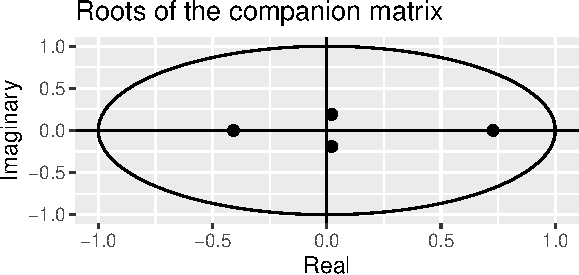
\includegraphics{02-final_presentation-V1_files/figure-beamer/stability.plot-1} \end{center}
\end{frame}

\begin{frame}{\textbf{5. CONSIDERAÇÕES FINAIS}}
\protect\hypertarget{considerauxe7uxf5es-finais}{}
\begin{itemize}
\tightlist
\item
  As variáveis que apresentaram significância simultaneamente no
  \emph{spread} e na rentabilidade foram:

  \begin{itemize}
  \tightlist
  \item
    Rentabilidade com uma e duas defasagens
  \item
    Despesas administrativas
  \item
    Receitas de operação de crédito
  \item
    Receitas de participação
  \item
    Selic over
  \item
    Velocidade da moeda.
  \end{itemize}
\end{itemize}
\end{frame}

\begin{frame}{\textbf{5. CONSIDERAÇÕES FINAIS}}
\protect\hypertarget{considerauxe7uxf5es-finais-1}{}
\begin{itemize}
\tightlist
\item
  Entre as principais variáveis determinantes que exercem influência
  direta no \emph{spread} estão, em ordem de peso:

  \begin{itemize}
  \tightlist
  \item
    Outras despesas operacionais,
  \item
    Receitas de operação de crédito,
  \item
    Outras receitas operacionais,
  \item
    Despesas administrativas,
  \item
    Velocidade da moeda
  \item
    Receita de serviços.
  \end{itemize}
\end{itemize}
\end{frame}

\begin{frame}{\textbf{5. CONSIDERAÇÕES FINAIS}}
\protect\hypertarget{considerauxe7uxf5es-finais-2}{}
\begin{itemize}
\tightlist
\item
  Entre as principais variáveis determinantes que exercem influência
  direta no \emph{spread} estão, em ordem de peso:

  \begin{itemize}
  \tightlist
  \item
    Rentabilidade de dois períodos anteriores,
  \item
    outras operações,
  \item
    depósitos de poupança,
  \item
    meios de pagamento M4,
  \item
    receita de participação,
  \item
    \emph{spread} de um período anterior
  \item
    compulsório.
  \end{itemize}
\end{itemize}
\end{frame}

\begin{frame}{\textbf{5. CONSIDERAÇÕES FINAIS}}
\protect\hypertarget{considerauxe7uxf5es-finais-3}{}
\begin{itemize}
\tightlist
\item
  Variáveis que apresentaram influência inversa no \emph{spread}, em
  ordem de peso estão:

  \begin{itemize}
  \tightlist
  \item
    Selic Over,
  \item
    IPCA,
  \item
    \emph{Spread} de dois períodos anteriores,
  \item
    Capital próprio
  \item
    Operação total do mercado
  \item
    Rentabilidade de um período anterior.
  \end{itemize}
\end{itemize}
\end{frame}

\begin{frame}{\textbf{5. CONSIDERAÇÕES FINAIS}}
\protect\hypertarget{considerauxe7uxf5es-finais-4}{}
\begin{itemize}
\tightlist
\item
  Variáveis que exercem influência direta com a rentabilidade, em ordem
  de peso, estão:

  \begin{itemize}
  \tightlist
  \item
    Rentabilidade de um e dois períodos anteriores,
  \item
    Velocidade da moeda,
  \item
    Impostos Indiretos e
  \item
    Despesas Administrativas.
  \end{itemize}
\end{itemize}
\end{frame}

\begin{frame}{\textbf{5. CONSIDERAÇÕES FINAIS}}
\protect\hypertarget{considerauxe7uxf5es-finais-5}{}
\begin{itemize}
\tightlist
\item
  Entre as variáveis que apresentaram influência inversa com a
  rentabilidade, em ordem de peso estão:

  \begin{itemize}
  \tightlist
  \item
    Imposto de renda
  \item
    Receita de operações de crédito
  \item
    Risco ponderado de crédito
  \item
    Operações de crédito
  \item
    Operações de financiamento
  \item
    Inadimplência
  \item
    Depósitos a vista
  \item
    Receitas de participações
  \item
    Selic over
  \end{itemize}
\end{itemize}
\end{frame}

\begin{frame}{\textbf{5. CONSIDERAÇÕES FINAIS}}
\protect\hypertarget{considerauxe7uxf5es-finais-6}{}
\begin{itemize}
\tightlist
\item
  Principal determinante simultâneo no \textbf{spread} e rentabilidade
  com relação direta

  \begin{itemize}
  \tightlist
  \item
    Velocidade da Moeda
  \end{itemize}
\end{itemize}

Quanto maior a velocidade da moeda, maior os níveis de \textbf{spread
ex-post} e rentabilidade
\end{frame}

\begin{frame}{\textbf{5. CONSIDERAÇÕES FINAIS}}
\protect\hypertarget{considerauxe7uxf5es-finais-7}{}
\begin{itemize}
\tightlist
\item
  Diante o resultado da pesquisa e da modelagem econométrica este estudo
  chega ao conceito que o \textbf{spread} e a rentabilidade bancária são
  definidos diante:

  \begin{itemize}
  \tightlist
  \item
    Conjunto de fatores endógenos remetendo as características
    operacionais de cada grupo e ou instituições
  \item
    Conjunto de fatores exógenos relacionados com a conjuntura social e
    econômica e de regulação.
  \end{itemize}
\end{itemize}
\end{frame}

\begin{frame}{\textbf{5. CONSIDERAÇÕES FINAIS}}
\protect\hypertarget{considerauxe7uxf5es-finais-8}{}
\textbf{ESTUDOS FUTUROS}

\begin{itemize}
\tightlist
\item
  Avaliação dos efeitos dos determinantes do \emph{spread} atuando
  simultaneamente sobre a taxa de aplicação, taxa de captação e
  rentabilidade bancária.
\item
  Orientação de trabalhar os dados no maior nível de desagregação
  possível para visualização do nível por tipo de tomador, tipo de
  operação, tipo de recurso, volume, prazo e nível de risco.
\end{itemize}
\end{frame}

\begin{frame}{\textbf{REFERÊNCIAS}}
\protect\hypertarget{referuxeancias}{}
ALMEIDA, F. D. Determinantes do spread bancário ex-post no Brasil: uma
análise de fatores micro e macroeconômicos. Brasíli: Universidade
Católica de Brasíl, 2013.

ALMONACID, Ruben D.; PASTORE, Affonso Celso. Uma nota sobre o
multiplicador da oferta monetária. Pesq. Plan. Econômico, IPEA, Rio de
Janeiro, 1976. Disponível em: \textless http:
//repositorio.ipea.gov.br/bitstream/11058/6813/1/PPE\_v6\_n2\_Uma\%20nota.pdf\textgreater.

ANDREWS, Donald W.K.; LU, Biao. Consistent model and moment selection
procedures for GMM estimation with application to dynamic panel data
models. Journal of Econometrics, MI, USA, 12 jul. 2000.
\end{frame}

\begin{frame}{\textbf{REFERÊNCIAS}}
\protect\hypertarget{referuxeancias-1}{}
ARELLANO, Manuel; BOND, Stephen. Some Tests of Specification for Panel
Data: Monte Carlo Evidence and an Application to Employment Equations.
Review of Economic Studies, v. 58, p.~277--297, 1991. Disponível em:
\textless{}\url{http://people.stern.nyu.edu/wgreene/}
Econometrics/Arellano-Bond.pdf\textgreater.

ARONOVICH, Selmo. Uma nota sobre os efeitos da inflação e do nível de
atividade sobre o spread bancário. Revista Brasileira de Economia, v.
48, n.~1, p.~125--40, 1994.

ASSAF NETO, Alexandre. Finanças corporativas e valor. São Paulo: Atlas,
2020. BABA, Y.; HENDRY, D. F.; STARR, R. M. The Demand for Ml in the USA
1960-1988.
\end{frame}

\begin{frame}{\textbf{REFERÊNCIAS}}
\protect\hypertarget{referuxeancias-2}{}
\_\_\_. Juros e Spread Bancário no Brasil. Brasília, 1999. Disponível
em: \url{https://www.bcb.gov.br/ftp/juros-spread1.pdf}. {[}S.l.{]},
1999. Brasília, 2000. Disponível em:
\textless{}\url{https://www.bcb.gov.br/ftp/}
jurospread112000.pdf\textgreater.

\_\_\_\_. Programação Monerária 2019. {[}S.l.{]}, 2019. Disponível em:
\url{https://www.bcb.gov.br/content/publicacoes/programacaomonetaria/pm-022019p.pdf}.

BACEN, SGS - Sistema Gerenciador de Séries Temporais. Agregados
Monetários. {[}S.l.: s.n.{]}. Disponível em:
\url{https://www3.bcb.gov.br/sgspub/consultarmetadados/consultarMetadadosSeries.do}?
method=consultarMetadadosSeriesInternet\&hdOidSerieSelecionada=27789.
Acesso em: 30/11/2020.
\end{frame}

\begin{frame}{\textbf{REFERÊNCIAS}}
\protect\hypertarget{referuxeancias-3}{}
BACEN, Sistema Gerenciador de Séries Temporais. Base Monetária. {[}S.l.:
s.n.{]}. Disponível em
\url{https://www3.bcb.gov.br/sgspub/consultarmetadados/}
consultarMetadadosSeries.do?method=consultarMetadadosSeriesInternet.
Acesso em: /12/2020.

\_\_\_\_\_. Meios de Pagamentos Ampliados. {[}S.l.: s.n.{]}. Disponível
em:
\url{https://www3.bcb.gov.br/sgspub/consultarmetadados/consultarMetadadosSeries.do}?
method=consultarMetadadosSeriesInternet\&hdOidSerieSelecionada=27810.
Acesso em 12/05/2020.

BANK, WORLD; IMF. Financial sector Assessment: a handbook. Washington
DCo: The World Bank, 2005. Disponível em:
\textless{}\url{http://documents1.worldbank.org/curated/en/}
306701468337879923/pdf/337970rev0Fina10Assessment01PUBLIC1.pdf\textgreater.
\end{frame}

\begin{frame}{\textbf{REFERÊNCIAS}}
\protect\hypertarget{referuxeancias-4}{}
BINDER, Michael; HSIAO, Cheng; PESARAN, M. Hashem. Estimation and
Inference in Short Panel Vector Autoregressions with Unit Roots and
Cointegration. Econometric Theory, Cambridge University Press, v. 21,
n.~4, p.~795--837, 2005. ISSN 02664666, 14694360. Disponível em:
\url{http://www.jstor.org/stable/3533397}.

BLUNDELL, Richard; BOND, Stephen. Initial conditions and moment
restrictions in dynamic panel data models. Journal of Econometrics, v.
87, n.~1, p.~115--143, 1998. Disponível em:
\url{https://www.ucl.ac.uk/~uctp39a/Blundell-Bond-1998.pdf}.

BONTEMPI, Maria Elena; MAMMI, Irene. Implementing a strategy to reduce
the instrument count in panel GMM. The Stata Journal, v. 15, n.~4,
p.~1075--1097, 12 jul. 2000.
\end{frame}

\begin{frame}{\textbf{REFERÊNCIAS}}
\protect\hypertarget{referuxeancias-5}{}
BORDO, M. D; L., JONUNG; L., SIKLOS P. Institutional and the Velocity of
Money: a century of evidence. Economic Inquiry, p.~710--724, 1997.

BRASIL. CONSTITUIÇÃO DA REPÚBLICA FEDERATIVA DO BRASIL DE 1988. Diário
Oficial da República Federativa do Brasil, Brasília, DF, 5 out. 1988.
Disponível em:
\url{http://www.planalto.gov.br/ccivil_03/constituicao/constituicao.htm}.
Acesso em: 7 set. 2020.

\_\_\_\_. DECRETO No 1.455. Diário Oficial da República Federativa do
Brasil, Brasília, DF, 30 dez. 1905. Disponível em:
\textless{}\url{https://www2.camara.leg.br/legin/fed/decret/1900-1909/decreto-1455-30-dezembro-}
1905-582773-publicacaooriginal-105568-pl.html\textgreater. Acesso em: 5
set. 2020.
\end{frame}

\begin{frame}{\textbf{REFERÊNCIAS}}
\protect\hypertarget{referuxeancias-6}{}
\_\_\_\_\_. DECRETO No 14.728. Diário Oficial da República Federativa do
Brasil, Brasília, DF, 16 mar. 1921. Disponível em:
\textless{}\url{https://www2.camara.leg.br/legin/fed/decret/1920-1929/decreto-14728-16-marco-}
1921-504798-publicacaooriginal-1-pe.html\textgreater. Acesso em: 15 mar.
2021. \_\_\_\_\_. DECRETO-LEI No 759, DE 12 DE AGOSTO DE 1969. Diário
Oficial da República Federativa do Brasil, Brasília, DF, 12 ago. 1969.
Disponível em:
\url{http://www.planalto.gov.br/ccivil_03/decreto-lei/del0759.htm}.
Acesso em: 4 set. 2020.
\end{frame}

\begin{frame}{\textbf{REFERÊNCIAS}}
\protect\hypertarget{referuxeancias-7}{}
\_\_\_\_\_. Lei no 4.595, de 31 de dezembro de 1964. Diário Oficial da
República Federativa do Brasil, Brasília, DF, 31 dez. 1964. Disponível
em: \url{http://www.planalto.gov.br/ccivil_03/leis/L4595.htm}. Acesso
em: 4 set. 2020.

BROCK, Philip L.; ROJAS SUAREZ, Liliana. Understanding the behavior of
bank spreads in Latin America. Journal of Development Economics, v. 63,
n.~1,p.~113--134, 2000. Disponível em:
\url{https://EconPapers.repec.org/RePEc:eee:deveco:v:63:y:2000:i:1:p:113-134}.

CAMARGO, Patrícia Olga. A evolução recente do setor bancário no Brasik.
São Paulo: Cultura Acadêmica, 2009.
\end{frame}

\begin{frame}{\textbf{REFERÊNCIAS}}
\protect\hypertarget{referuxeancias-8}{}
CAMPELLO, Mauro Luiz Costa; BRUNSTEIN, Israel. UMA ANÁLISE DA
COMPETITIVIDADE DOS BANCOS DE VAREJO NO BRASIL. REVISTA GESTÃO DA
PRODUÇÃO OPERAÇÕES E SISTEMAS, Unesp, v. 1, n.~1, p.~83--99, 2005.

CARDOSO, Renato Fragelli; KOYAM, Sérgio Mikioa. A CUNHA FISCAL SOBRE A
INTERMEDIAÇÃO FINANCEIRA. In: {[}s.l.{]}: Banco Central do Brasil, 1999.
P. 129--158.

CMN. Resolução CMN 2.624, de 1999. Diário Oficial da República
Federativa do Brasil, Brasília, DF, 29 jul. 1999. Disponível em:
\textless{}\url{https://www.bcb.gov.br/pre/normativos/busca/downloadNormativo.asp?arquivo=}
/Lists/Normativos/Attachments/45083/Res\_2624\_v1\_O.pdf\textgreater.
Acesso em: 4 set. 2020.
\end{frame}

\begin{frame}{\textbf{REFERÊNCIAS}}
\protect\hypertarget{referuxeancias-9}{}
\_\_\_\_\_. Resolução CMN 3.426, de 2006. Diário Oficial da República
Federativa do Brasil, Brasília, DF, 26 dez. 2006. Disponível em:
\url{https://www.bcb.gov.br/pre/normativos/res/1976/pdf/res_0394_v13_P.pdf}.
Acesso em: 4 set. 2020.

\_\_\_. Resolução CMN 394, de 1976. Diário Oficial da República
Federativa do Brasil, Brasília, DF, 20 out. 1976. Disponível em:
\textless{}\url{https://www.bcb.gov.br/pre/normativos/res/1976/pdf/res_0394_v13_P}
pdf\textgreater. Acesso em: 4 set. 2020.

\_\_\_\_. Resolução No 1.524 de 1988. Diário Oficial da República
Federativa do Brasil, Brasília, DF, 24 set. 1988. Disponível em:
\url{https://www.bcb.gov.br/pre/normativos/res/1988/pdf/res_1524_v8_P.pdf}.
Acesso em: 24 fev. 2017.
\end{frame}

\begin{frame}{\textbf{REFERÊNCIAS}}
\protect\hypertarget{referuxeancias-10}{}
\_\_\_\_\_. Resolução no 2.099. Diário Oficial da República Federativa
do Brasil, Brasília DF, 17 ago. 1994. Disponível em:
\url{https://www.bcb.gov.br/pre/normativos/res/1994/pdf/res_2099_v1_O.pdf}.
Acesso em: 4 set. 2020.

CÓRDOBA, Miguel. Análisis Financiero de los Mercados Monetarios y de
Valores. Madrid: Saraiva, 1996.

COSTA, Ana Carla Abrão; NAKANE, Márcio I. Spread bancário no Brasil:
dois esclarecimentos e duas constatações. Tecnologia de Crédito, 2004.
\end{frame}

\begin{frame}{\textbf{REFERÊNCIAS}}
\protect\hypertarget{referuxeancias-11}{}
COSTA NETO, Yttrio Corrêa da. Bancos oficiais no Brasil: origem e
aspectos de seu desenvolvimento. Brasília: Banco Central do Brasil,
2004. Disponível em:
\url{https://www.bcb.gov.br/htms/public/BancosEstaduais/livros_bancos_oficiais.pdf}.

COUTO, Rodrigo Luís Rosa. Metodologia de avaliação da capacidade de
geração de resultados de instituições financeiras. {[}S.l.{]}, 2002.
(Notas Técnicas do Banco Central do Brasil). Disponível em:
\textless Dispon\%C3\%ADvel\%20em\%20\%5Curl\%7Bhttps://www.bcb.gov.br/pec/notastecnicas/port/2002nt26avalgeracaoresultp.pdf\%7D\%
20Acesso\%20em:\%2020/11/2020\textgreater.

DANTAS, José A. Determinantes do spread bancário ex post no mercado
brasileiro. REV. ADM. MACKENZIE, UNIVERSIDADE PRESBITERIANA MACKENZIE,
v. 13, n.~4, p.~48--74, 2012.
\end{frame}

\begin{frame}{\textbf{REFERÊNCIAS}}
\protect\hypertarget{referuxeancias-12}{}
DEMIRGÜÇ-KUNT, Ash; HUIZINGAGA, Harry. Determinants of commercial bank
interest margins and profitability: some international evidence. The
World Bank Economic Review, v. 13, p.~379--408, 1 mai. 1999. Disponível
em: \textless https:
//citeseerx.ist.psu.edu/viewdoc/download?doi=10.1.1.194.3108\&rep=rep1\&type=pdf\textgreater.
Acesso em: 8 set. 2020.

DICK, Astrid. Banking Spreads in Central America: Evolution, Structure,
and Behavior. HIID Development Discussion Papers, Harvard Institute for
International Development, Cambridge, 1999.

DURIGAN, Junior et al.~Fatores macroeconômicos, indicadores industriais
e o spread bancário no Brasil. Revista de Ciências da Administração -
RCA, 2018. DOI: 10.5007/2175-8077.2018v20n51p26.
\end{frame}

\begin{frame}{\textbf{REFERÊNCIAS}}
\protect\hypertarget{referuxeancias-13}{}
FARIA, Miguel Figueira de Faria; MENDES, José Amado. Dicionário de
História Empresarial Portuguesa, Séculos XIX e XX. Porto: INCM, 2014. v.
I.

FIPECAFI. ESTUDO SOBRE A APURAÇÃO DO SPREAD DA INDÚSTRIA BANCÁRIA.
{[}S.l.{]}, 2005. Disponível em:
\url{https://www.bcb.gov.br/ftp/jurospread112000.pdf}.

FRIEDMAN, M.; SCHWARTZ, A. J. A monetary history of the United States,
1867 -- 1960. Princeton: Princeton University Press, 1963.
\end{frame}

\begin{frame}{\textbf{REFERÊNCIAS}}
\protect\hypertarget{referuxeancias-14}{}
\_\_\_\_\_. Monetary Trends in the United States and the United Kingdom
Their Relation to Income, Prices, and Interest Rates, 1867-1975.
Chicago: University of Chicago Press for NBER, 1982.

GRAHAM, Benjamin; MEREDITH, Spencer B. A interpretação das demonstrações
financeiras. 3. ed.~São Paulo: Saraiva, 2012.

GUIMARÃES, Carlos Gabriel. O Estado Imperial brasileiro e os bancos
estrangeiros: o caso do London and Brazilian Bank (1862-1871). Anais do
XXVI Simpósio Nacional de História -- AUHNP São Paulo, julho 2011, 2011.
Disponível em: \textless{}\url{http://www.snh2011.anpuh.org/resources}
/anais/14/1298818435\_ARQUIVO\_ TextoLBBnovo.pdf\textgreater.
\end{frame}

\begin{frame}{\textbf{REFERÊNCIAS}}
\protect\hypertarget{referuxeancias-15}{}
HAFER, R. W.; JANSEN, D. W. The Demand for Money in the United States:
Evidence from Cointegration Test. Journal of Money, Credit, and Banking,
p.~155--68, 1991.

HENDRY, David F.; MIZON, Grayham E. Serial Correlation as a Convenient
Simplification, Not a Nuisance: A Comment on a Study of the Demand for
Money by the Bank of England. The Economic Journal, {[}Royal Economic
Society, Wiley{]}, v. 88,n.~351, p.~549--563, 1978. ISSN 00130133,
14680297. Disponível em: \url{http://www.jstor.org/stable/2232053}.HILL,
R. Carter. Economertia. 3. ed.~São Paulo: Saraiva, 2010.

HO, Thomas S. Y.; SAUNDERS, Anthony. The Determinants of Bank Interest
Margins: Theory and Empirical Evidence. Journal of Financial and
Quantitative Analysis,v. 16, n.~4, p.~581--600, 1981. Disponível
em:\url{https://EconPapers.repec.org/RePEc:cup:jfinqa:v:16:y:1981:i:04:p:581-600_00}.
\end{frame}

\begin{frame}{\textbf{REFERÊNCIAS}}
\protect\hypertarget{referuxeancias-16}{}
HOLTZ-EAKIN, D.; NEWEY, W.; ROSEN, H.S. Estimating vector
autoregressions with panel data. Econometrica, v. 56, n.~1371-1395,
1988. Disponível em: \textless6\textgreater.

JAMES, Gareth et al.~An Introduction to Statistical Learning. 8. ed.~New
York: Springer, 2017.

KAPETANIOS, G. A bootstrap procedure for panel data sets with many
cross-sectional units. The Econometrics Journal, {[}Royal Economic
Society, Wiley{]}, v. 11, n.~2,p.~377--395, 2008. ISSN 13684221,
1368423X. Disponível em: \url{http://www.jstor.org/stable/23116081}.
\end{frame}

\begin{frame}{\textbf{REFERÊNCIAS}}
\protect\hypertarget{referuxeancias-17}{}
KLEIN, Michael A. A Theory of the Banking Firm. Journal of Money, Credit
and Banking, Ohio State University Press, v. 3, n.~2, p.~205--218, mai.
1971. Disponível em: \url{http://www.jstor.org/stable/1991279}.

LEITE, J. C. Tecnologia e organizações: um estudo sobre os efeitos da
introdução de novas tecnologias no setor bancário brasileiro. 1996. Tese
(Doutorado) -- São Paulo.

LEVINE, Ross. Financial Development and Economic Growth: Views and
Agenda. Journal of Economic Literature, American Economic Association,
v. 35, n.~2,p.~688--726, 1997. ISSN 00220515. Disponível em:
\url{http://www.jstor.org/stable/2729790}.
\end{frame}

\begin{frame}{\textbf{REFERÊNCIAS}}
\protect\hypertarget{referuxeancias-18}{}
MAFFILI, Dener William; BRESSAN, Aureliano Angel; SOUZA, Antônio Artur
da. Estudo da Rentabilidade dos Bancos Brasileiros de Varejo no Período
de 1999 a 2005. Contabilidade Vista e Revista, SI, v. 238, n.~2,
p.~117--138, 12 mai. 2009. Disponível em:
\textless Dispon\%C3\%ADvel\%20em\%20\%5Curl\%7Bhttps:
//www.imf.org/external/pubs/ft/op/238/index.htm\%7D\%20Acesso\%20em:
\%2017\%20fev.\%202021\textgreater.

MAGALHÃES-TIMOTIO, João G. RELAÇÃO ENTRE INDICADORES CONTÁBEIS E O
SPREAD EX-POST DOS BANCOS BRASILEIROS. RACEF -- Revista de
Administração, Contabilidade e Economia da Fundace, v. 9, n.~2,
p.~31--44, 2018.

MATOS, Orlando Carneiro de. Inter-relações entre Desenvolvimento
Financeiro, Exportações e Crescimento Econômico: Análise da Experiência
Brasileira. In: NOTAS Técnicas do Banco Central do Brasil. Brasília:
BCB, 2003. Disponível em:
\textless{}\url{https://www.bcb.gov.br/content/publicacoes/notastecnicas/2003nt40Inter-}
relentreDesenvFinanp.pdf\textgreater.
\end{frame}

\begin{frame}{\textbf{REFERÊNCIAS}}
\protect\hypertarget{referuxeancias-19}{}
MILLER, Stephen. Monetary Dynamics: An Application of Cointegration and
Error-Correction Modeling. Journal of Money, Credit and Banking, v. 23,
n.~2, p.~139--54, 1991. Disponível em:
\url{https://EconPapers.repec.org/RePEc:mcb:jmoncb:v:23:y:1991:i:2:p:139-54}.

NEVES JÚNIOR, Idalberto José das; SOARES RIBEIRO, Francilanes;MENDES,
Frederico. EFICIÊNCIA OPERACIONAL: UMA ANÁLISE EXPLORATÓRIA DOS 50
MAIORES BANCOS BRASILEIROS PELO RANKING BACEN. 4o Congresso USP de
Iniciação Científica em Contabilidade, USP, 2007. Disponível em:
\url{https://intercostos.org/documentos/apellidos/Das\%20Neves\%201.pdf}.
OREIRO, José Luís da Costa; PAULO, Luiz Fernando de. Determinantes
macroeconômicos do spread bancário no Brasil: teoria e evidência
recente. Economia Aplicada, v. 10, n.~4, p.~609--634, 2006.
\end{frame}

\begin{frame}{\textbf{REFERÊNCIAS}}
\protect\hypertarget{referuxeancias-20}{}
REY, Letícia Dias. Spread Bancário Brasileiro: um indicador de excessos?
Insper, 2017. Disponível em:
\textless{}\url{http://dspace.insper.edu.br/xmlui/bitstream/handle/11224/1799/Let\%}
C3\%ADcia\%20Dias\%20Rey\_Trabalho.pdf?sequence=1\textgreater.

ROVER, Suliani; TOMAZZIA, Eduardo Cardeal; FÁVER, Luiz Paulo.
Determinantes Econômico-Financeiros e Macroeconômicos da Rentabilidade:
Evidências Empíricas do Setor Bancário Brasileo. Revista Brasileira de
Economia, XXXV Encontro da ANPAD, 2011.

SARGAN, Denis J. Wages and Prices in the U.K.: A Study in Econometric
Methodology. in Econometric Analysis for National Economic Planning,
Paul Hart, Gary Mills and John K. Whitaker (eds) Colston Papers1,
Butterworths, London, v. 16, p.~25--54, 1964.
\end{frame}

\begin{frame}{\textbf{REFERÊNCIAS}}
\protect\hypertarget{referuxeancias-21}{}
SIGMUND, Michael; FERSTL, Robert. Panel Vector Autoregression inR with
the Package panelvar, 2008. Disponível em:
\textless{}\url{https://www.researchgate.net/publication/}
312165764\_Panel\_Vector\_Autoregression\_in\_R\_with\_the\_Package\_Panelvar\textgreater.

SINGH, Anoop et al.~Stabilization and Reform in Latin America: A
Macroeconomic Perspective on the Experience Since the Early 1990s.
Occasional Paper, International Monetary Fund, v. 238, n.~2, fev. 2005.
Disponível em:
\url{https://www.imf.org/external/pubs/ft/op/238/index.htm}.

SOUZA, Rodrigo Mendes Leal de. Estrutura e determinantes do spread
bancário no Brasil:uma resenha comparativa da literatura empírica. Rio
de Janeiro: Universidade do Estado do Rio de Janeiro, 2006.
\end{frame}

\begin{frame}{\textbf{REFERÊNCIAS}}
\protect\hypertarget{referuxeancias-22}{}
VASCONCELLOS, Marco Antonio Sandoval de. Macroeconomia. 3. ed.~São
Paulo: Atlas, 2001.

VIEIRA, Heleno Piazentini; PEREIRA, Pedro Luiz Valls. Velocidade da
moeda e ciclos econômicos no Brasil, 1900-2016. Insper Working Paper,
New York, NY, p.~1--38, 2016. Disponível em:
\textless{}\url{https://www.insper.edu.br/wp-content/uploads/2018/10/Velocidade-}
moeda-ciclos-economicos-Brasil.pdf\textgreater.

ZIVOT, Eric; WANG, Jiahui. Vector Autoregressive Models for Multivariate
Time Series. In: Modeling Financial Time Series with S-Plus. Springer,
New York, NY, p.~369--413, 2003. Disponível em:
\url{https://doi.org/10.1007/978-0-387-21763-5_11}.
\end{frame}

\begin{frame}{\textbf{AGRADECIMENTOS}}
\protect\hypertarget{agradecimentos}{}
\textbf{OBRIGADO}
\end{frame}

\begin{frame}{\textbf{REFERÊNCIAS}}
\protect\hypertarget{referuxeancias-23}{}
\hypertarget{refs}{}
\begin{CSLReferences}{1}{0}
\leavevmode\vadjust pre{\hypertarget{ref-andrews-lu:2001}{}}%
Andrews, Donald W. K., and Biao Lu. 2000. {``Consistent Model and Moment
Selection Procedures for GMM Estimation with Application to Dynamic
Panel Data Models.''} \emph{Journal of Econometrics}, July.

\leavevmode\vadjust pre{\hypertarget{ref-BCB:2000}{}}%
BACEN. 2000. {``Juros e Spread Bancário No Brasil.''} Brasília: Banco
Central do Brasil.
\url{https://www.bcb.gov.br/ftp/jurospread112000.pdf}.

\leavevmode\vadjust pre{\hypertarget{ref-BCB:2016}{}}%
---------. 2016. {``Juros e Spread Bancário.''} Brasília: Banco Central
do Brasil.

\leavevmode\vadjust pre{\hypertarget{ref-WB:2005}{}}%
BANK, WORLD, and IMF. 2005. \emph{Financial Sector Assessment: A
Handbook}. Washington DCo: The World Bank.
\url{http://documents1.worldbank.org/curated/en/306701468337879923/pdf/337970rev0Fina10Assessment01PUBLIC1.pdf}.

\leavevmode\vadjust pre{\hypertarget{ref-blundelbond:1998}{}}%
Blundell, Richard, and Stephen Bond. 1998. {``Initial Conditions and
Moment Restrictions in Dynamic Panel Data Models.''} \emph{Journal of
Econometrics} 87 (1): 115--43.
\url{https://www.ucl.ac.uk/~uctp39a/Blundell-Bond-1998.pdf}.

\leavevmode\vadjust pre{\hypertarget{ref-bontempi:2015}{}}%
Bontempi, Maria Elena, and Irene Mammi. 2000. {``Implementing a Strategy
to Reduce the Instrument Count in Panel GMM.''} \emph{The Stata Journal}
15 (4): 1075--97.

\leavevmode\vadjust pre{\hypertarget{ref-dantas:2012}{}}%
Dantas, José A. 2012. {``Determinantes Do Spread Bancário Ex Post No
Mercado Brasileiro.''} \emph{REV. ADM. MACKENZIE} 13 (4): 48--74.

\leavevmode\vadjust pre{\hypertarget{ref-dick:1999}{}}%
Dick, Astrid. 1999. {``Banking Spreads in Central America: Evolution,
Structure, and Behavior.''} \emph{HIID Development Discussion Papers}.

\leavevmode\vadjust pre{\hypertarget{ref-hendry:1978}{}}%
Hendry, David F., and Grayham E. Mizon. 1978. {``Serial Correlation as a
Convenient Simplification, Not a Nuisance: A Comment on a Study of the
Demand for Money by the Bank of England.''} \emph{The Economic Journal}
88 (351): 549--63. \url{http://www.jstor.org/stable/2232053}.

\leavevmode\vadjust pre{\hypertarget{ref-levine:1997}{}}%
Levine, Ross. 1997. {``Financial Development and Economic Growth: Views
and Agenda.''} \emph{Journal of Economic Literature} 35 (2): 688--726.
\url{http://www.jstor.org/stable/2729790}.

\leavevmode\vadjust pre{\hypertarget{ref-timotio:2018}{}}%
Magalhães-Timotio, João G. 2018. {``RELAÇão ENTRE INDICADORES CONTÁBEIS
e o SPREAD EX-POST DOS BANCOS BRASILEIROS.''} \emph{RACEF -- Revista de
Administração, Contabilidade e Economia Da Fundace} 9 (2): 31--44.

\leavevmode\vadjust pre{\hypertarget{ref-matos:2003}{}}%
Matos, Orlando Carneiro de. 2003. {``Inter-Relações Entre
Desenvolvimento Financeiro, Exportações e Crescimento Econômico: Análise
Da Experiência Brasileira.''} In \emph{Notas Técnicas Do Banco Central
Do Brasil}. Brasília: BCB.
\url{https://www.bcb.gov.br/content/publicacoes/notastecnicas/2003nt40Inter-relentreDesenvFinanp.pdf}.

\leavevmode\vadjust pre{\hypertarget{ref-sargan:1964}{}}%
Sargan, Denis J. 1964. {``Wages and Prices in the u.k.: A Study in
Econometric Methodology.''} \emph{In Econometric Analysis for National
Economic Planning, Paul Hart, Gary Mills and John K. Whitaker (Eds)
Colston Papers1} 16: 25--54.

\leavevmode\vadjust pre{\hypertarget{ref-sigmund:2008}{}}%
Sigmund, Michael, and Robert Ferstl. 2008. {``Panel Vector
Autoregression inR with the Package Panelvar.''}
\url{https://www.researchgate.net/publication/312165764_Panel_Vector_Autoregression_in_R_with_the_Package_Panelvar}.

\leavevmode\vadjust pre{\hypertarget{ref-leal:2006}{}}%
Souza, Rodrigo Mendes Leal de. 2006. {``Estrutura e Determinantes Do
Spread Bancário No Brasil:uma Resenha Comparativa Da Literatura
Empírica.''} Rio de Janeiro: Universidade do Estado do Rio de Janeiro.

\leavevmode\vadjust pre{\hypertarget{ref-zivotwang:2003}{}}%
Zivot, Eric, and Jiahui Wang. 2003. {``Vector Autoregressive Models for
Multivariate Time Series. In: Modeling Financial Time Series with
s-Plus,''} 369--413. \url{https://doi.org/10.1007/978-0-387-21763-5_11}.

\end{CSLReferences}
\end{frame}

\end{document}
